\section*{\underline{PART C: Understanding Uncertainty from Sampling}}
\markboth{PART C: Understanding Uncertainty from Sampling}{}

\subsection*{Question 7: If we had selected another sample of repairs, would we obtain exactly the same mean repair time?}

No, if we selected another sample of repairs, we would not obtain exactly the same mean repair time due to sampling variability. Because each sample contains a different random subset of repair events, the calculated sample mean will naturally fluctuate from one sample to the next.

To quantify how much the sample mean repair time can vary when drawn from the same population, we performed a simulation by drawing 1,000 random samples, each with a sample size of $n = 50$, from our dataset. The results of this sampling distribution are summarized below:

\begin{itemize}
    \item \textbf{Number of samples:} 1000
    \item \textbf{Sample size ($n$):} 50
    \item \textbf{Lowest sample mean:} 9.62 minutes
    \item \textbf{Highest sample mean:} 29.39 minutes
    \item \textbf{Mean of sample means:} 16.32 minutes
    \item \textbf{Standard error:} 3.23 minutes
\end{itemize}

As observed, the sample means fluctuated significantly, ranging from 9.62 minutes up to 29.39 minutes, yielding a standard error of 3.23 minutes. The distribution of these 1,000 sample means is visualized in Figure \ref{fig:sampling_dist}. 

\begin{figure}[H]
    \centering
    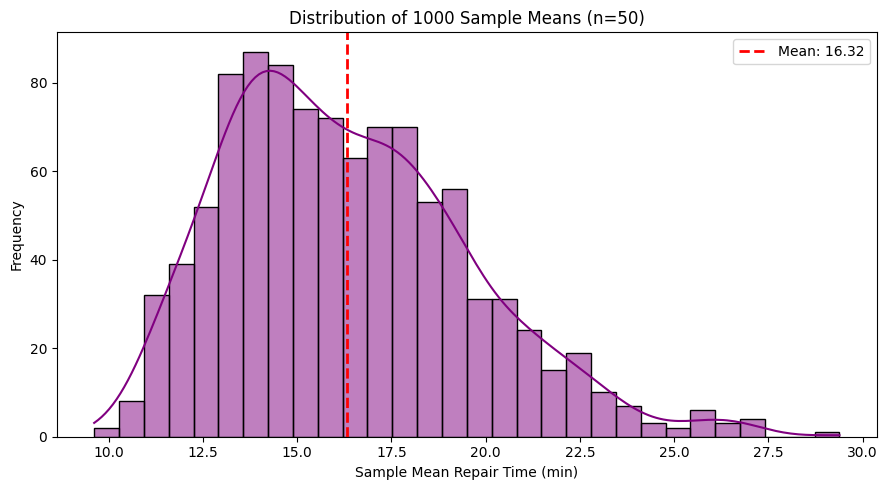
\includegraphics[width=0.85\linewidth]{figures/freq3.png}
    \caption{Distribution of 1000 Sample Means ($n=50$). The dashed red line indicates the mean of the sample means at 16.32 minutes.}
    \label{fig:sampling_dist}
\end{figure}

\subsection*{Question 8: How does increasing the sample size affect the variability of the sample mean and the precision of our estimate?}

Increasing the sample size directly reduces the variability of the sample mean, thereby increasing the precision of our estimate for the true population mean. This occurs because larger samples provide more information and are less sensitive to extreme outliers present in the heavy right-skewed tail of our downtime data. 

To demonstrate this, we simulated sampling distributions across three different sample sizes ($n = 10, 50, \text{ and } 200$). The resulting standard errors (SE) are:

\begin{itemize}
    \item \textbf{Standard Error ($n=10$):} 7.19 minutes
    \item \textbf{Standard Error ($n=50$):} 3.20 minutes
    \item \textbf{Standard Error ($n=200$):} 1.59 minutes
\end{itemize}

As the sample size increases, the standard error shrinks. Notably, when we quadruple the sample size from $n=50$ to $n=200$, the standard error approximately halves (from 3.20 to 1.59), which aligns perfectly with the Central Limit Theorem's definition of standard error ($\sigma / \sqrt{n}$). 

This reduction in variability is visually evident in Figure \ref{fig:sample_size_comparison}, where the density curves become progressively narrower and more concentrated around the true mean as $n$ increases.

\begin{figure}[H]
    \centering
    \begin{minipage}{0.48\textwidth}
        \centering
        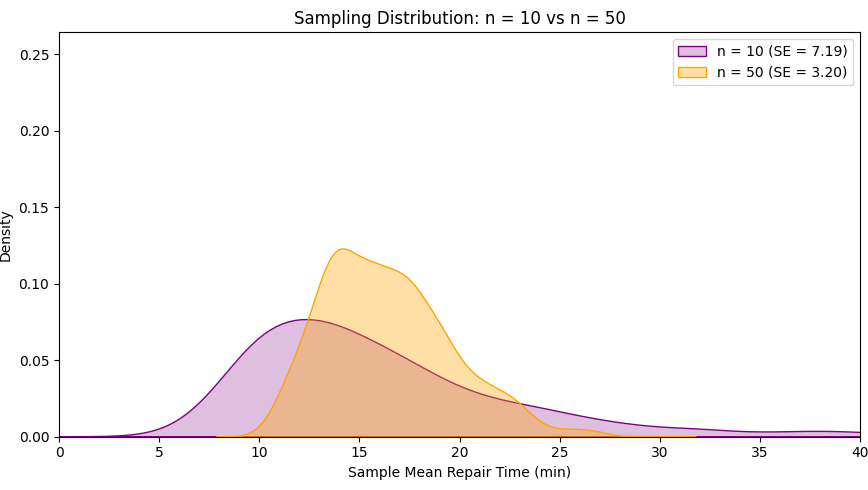
\includegraphics[width=\linewidth]{figures/samplesize1.png}
        \caption{Sampling Distribution ($n=10$ vs $n=50$)}
        \label{fig:n10_vs_n50}
    \end{minipage}\hfill
    \begin{minipage}{0.48\textwidth}
        \centering
        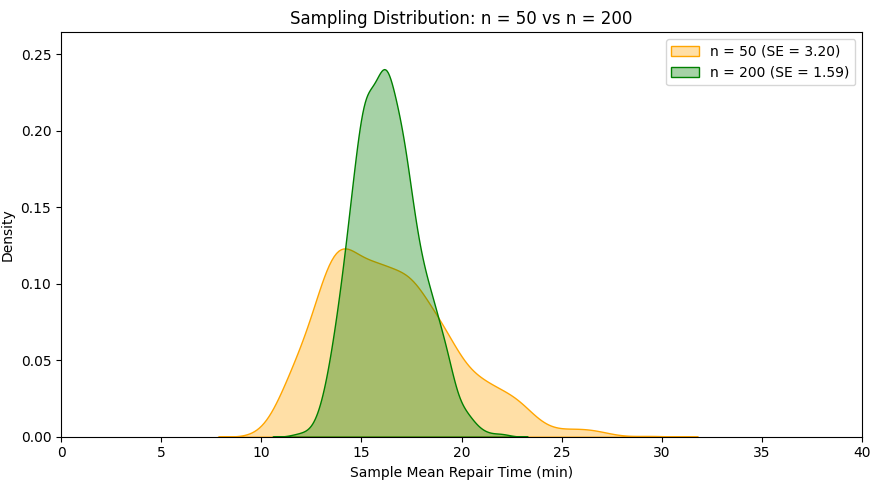
\includegraphics[width=\linewidth]{figures/samplesize2.png}
        \caption{Sampling Distribution ($n=50$ vs $n=200$)}
        \label{fig:n50_vs_n200}
    \end{minipage}
\end{figure}